\documentclass[serif,mathserif]{beamer}
\usepackage{amsmath, amsfonts, epsfig, xspace}
\usepackage{algorithm,algorithmic}
\usepackage{pstricks,pst-node}
\usepackage{multimedia}
\usepackage[normal,tight,center]{subfigure}
\setlength{\subfigcapskip}{-.5em}
\usepackage{beamerthemesplit}
\usetheme{lankton-keynote}

\author{Ben Keller}

\title[Molecular Cloud Turbulence\hspace{2em}\insertframenumber/\inserttotalframenumber]{Turbulence in
Molecular Clouds}

\date{Feb. 26 2013} %leave out for today's date to be insterted

\institute{Physics 785}

\begin{document}

\maketitle

% \section{Introduction}  % add these to see outline in slides

\begin{frame}
  \frametitle{Introduction}
  \begin{itemize}
  \item Background and Basic Theory\pause
  \item Observational Evidence\pause
  \item Origins of Turbulence\pause
  \item Implications of Molecular Cloud Physics
  \end{itemize}
\end{frame}

% \section{Main Body} % add these to see outline in slides

\begin{frame}
  \frametitle{Molecular Clouds}
  \begin{itemize}
	  \item Cold ($<100K$) and dense ($>100 cm^{-3}$)
	  \item Chemically and Structurally Complex
	  \item Stellar Nurseries
  \end{itemize}
\end{frame}

\begin{frame}
  \frametitle{Molecular Clouds}
  \begin{figure}[t]
	\centering
	\includegraphics[width=11cm]{figures/rho_oph}
  \end{figure}
\end{frame}

\begin{frame}
  \frametitle{Kolmogorov's 1941 Theory}
  We begin by defining...
  \begin{itemize}
	  \item Assume isotropic, homogeneous turbulence
  \item Two key hypotheses relating $\nu$, $\epsilon$
    \begin{equation*}
		\eta = \nu^{3/4}\epsilon^{1/4}
    \end{equation*}
    \begin{equation*}
		\sigma = \sqrt{\nu/\epsilon}
    \end{equation*}
  \item Characteristic Energy Spectrum
    \begin{equation*}
		E(k) \propto \epsilon^{2/3}k^{-5/3}
    \end{equation*}
  \end{itemize}
\end{frame}

\begin{frame}
	\frametitle{Not the whole story...}
  \begin{figure}[t]
	\centering
	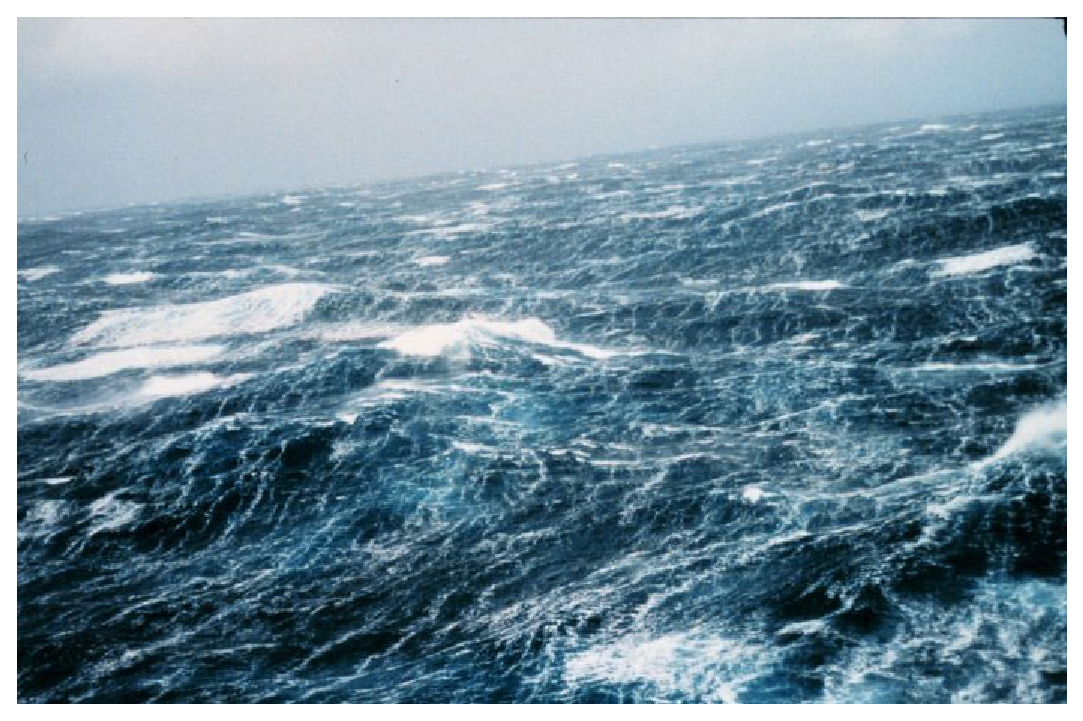
\includegraphics[width=8cm]{figures/turbulence1}
  \end{figure}
\end{frame}

\begin{frame}
	\frametitle{Real ISM Turbulence is...}
  \begin{itemize}
	  \item Compressible! (Turbulence in molecular clouds is often supersonic)
	  \item Magnetized! (Molecular clouds have magnetic fields of a few 10s $\mu
		  G$
  \end{itemize}
\end{frame}

\begin{frame}
	\frametitle{MHD Turbulence}
  \begin{itemize}
	  \item Isotropy broken
	  \item Power-law spectrum (-3/2 slope)
	  \item Decays in roughly a crossing time
	  \item Effects vs. hydrodynamic turbulence may be small
  \end{itemize}
\end{frame}

\begin{frame}
	\frametitle{MHD Turbulence promotes filament/sheet growth}
  \begin{figure}[t]
	\centering
	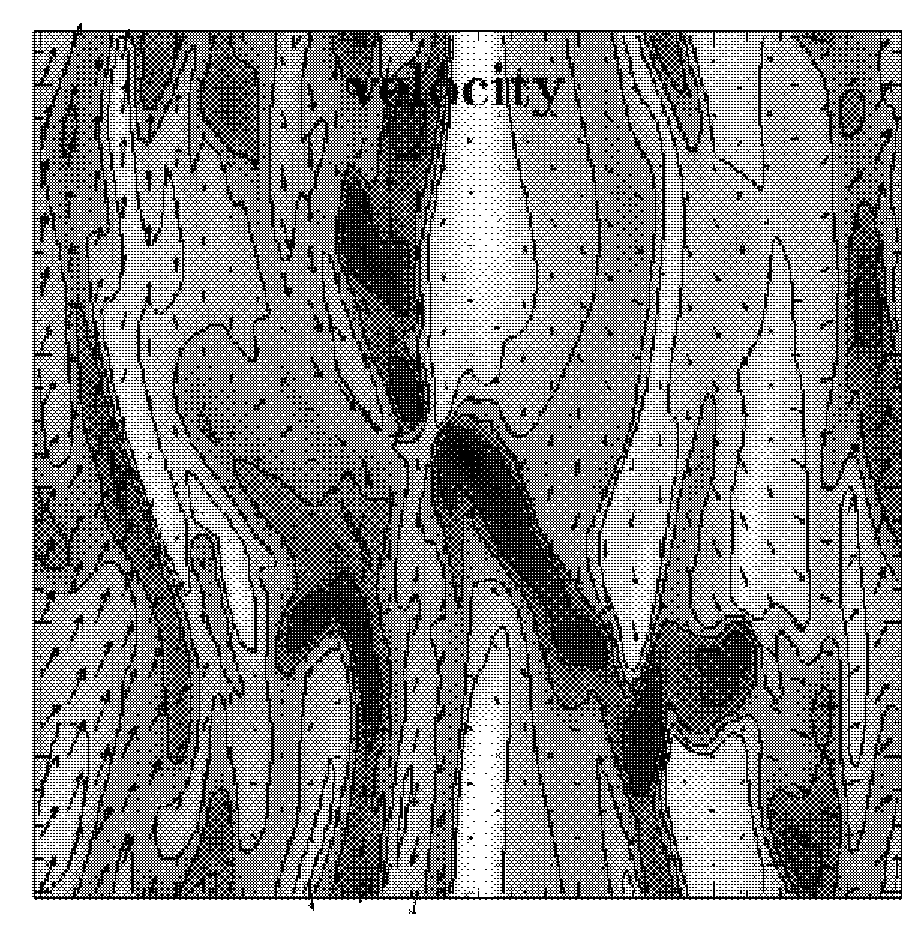
\includegraphics[width=5cm]{figures/MHD_v}
	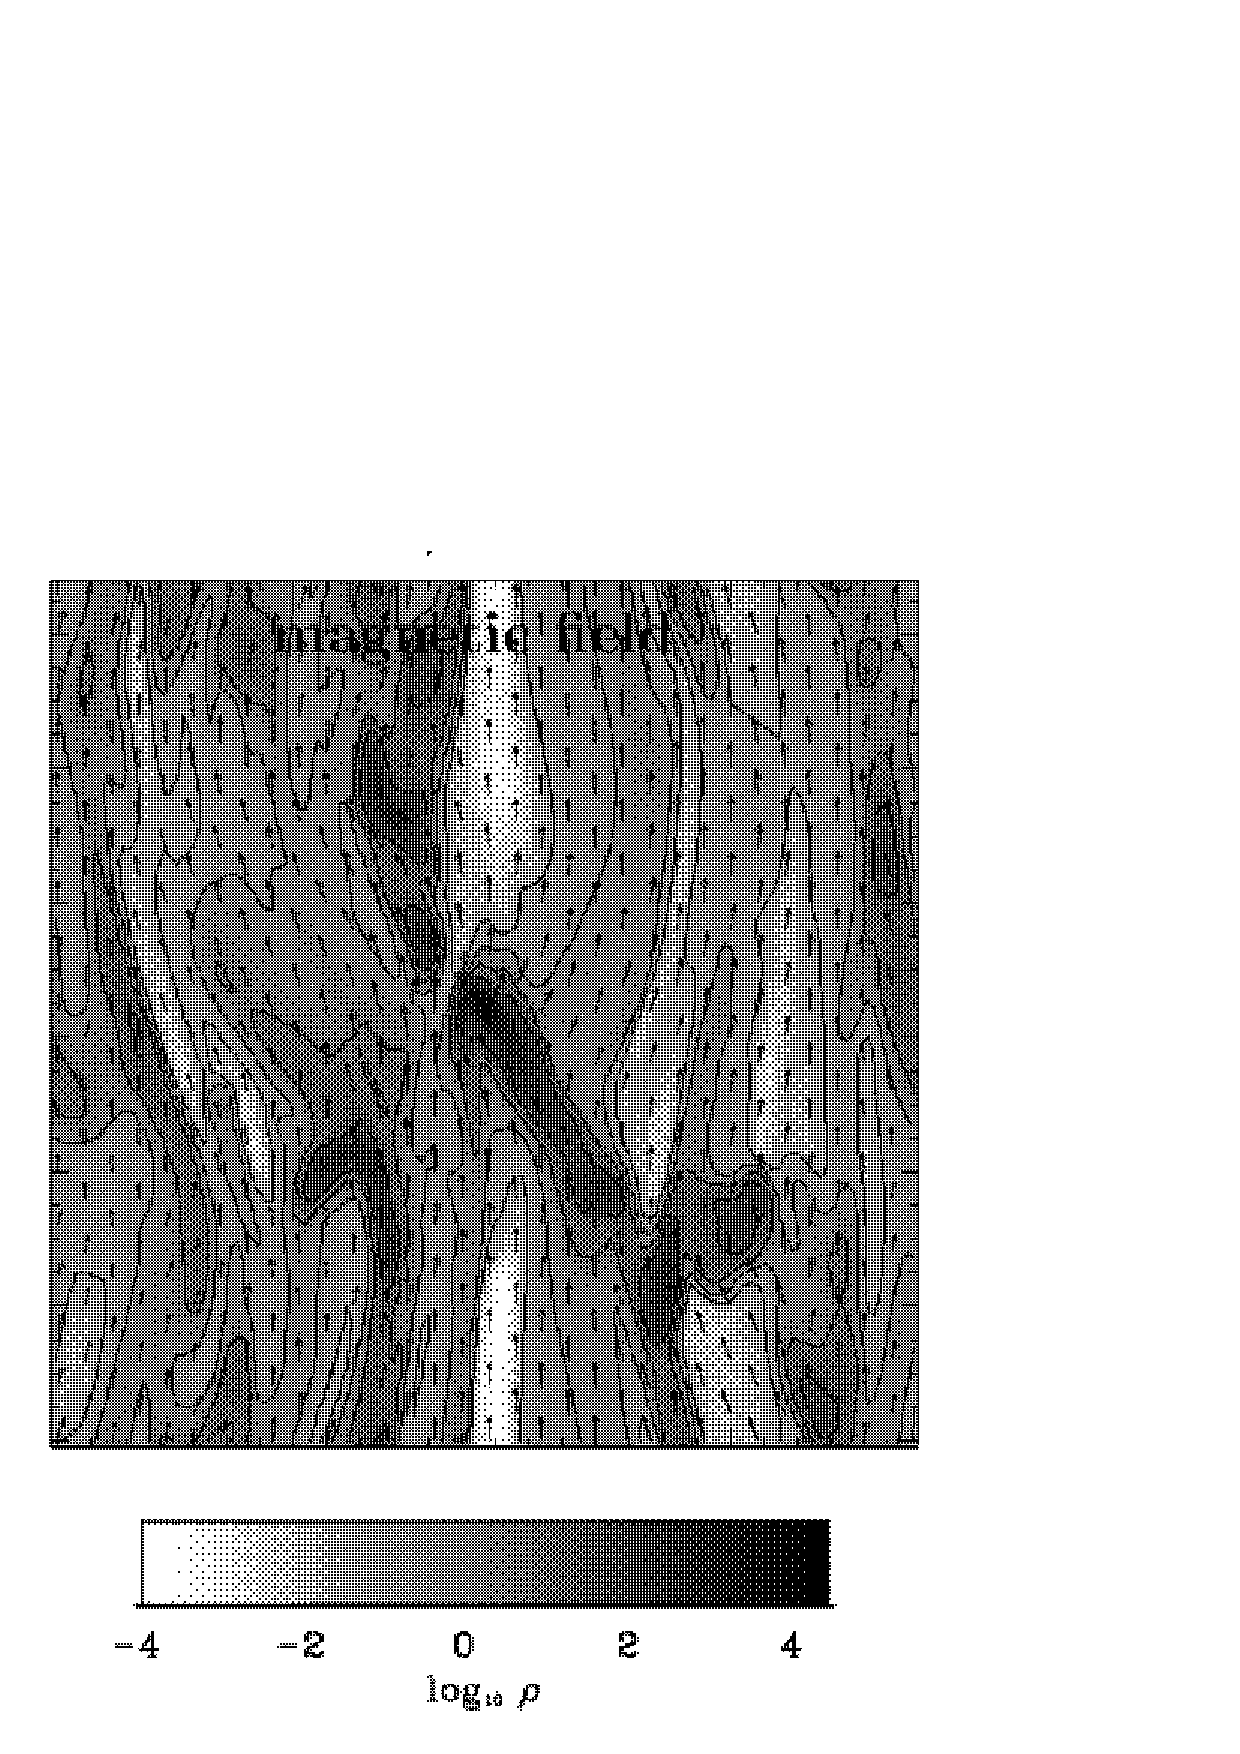
\includegraphics[width=5cm]{figures/MHD_B}
  \end{figure}
\end{frame}

\begin{frame}
	\frametitle{Observational Evidence of Turbulence}
	\begin{itemize}
		\item Real-space Kolmogorov spectrum
    \begin{equation*}
		\sigma \propto L^{1/3}
    \end{equation*}
		\item Power spectrum of density field
		\item Larson's 1979 and 1981 CO Observations
	\end{itemize}
\end{frame}

\begin{frame}
	\frametitle{Larson's First Law}
  \begin{figure}[t]
	\centering
	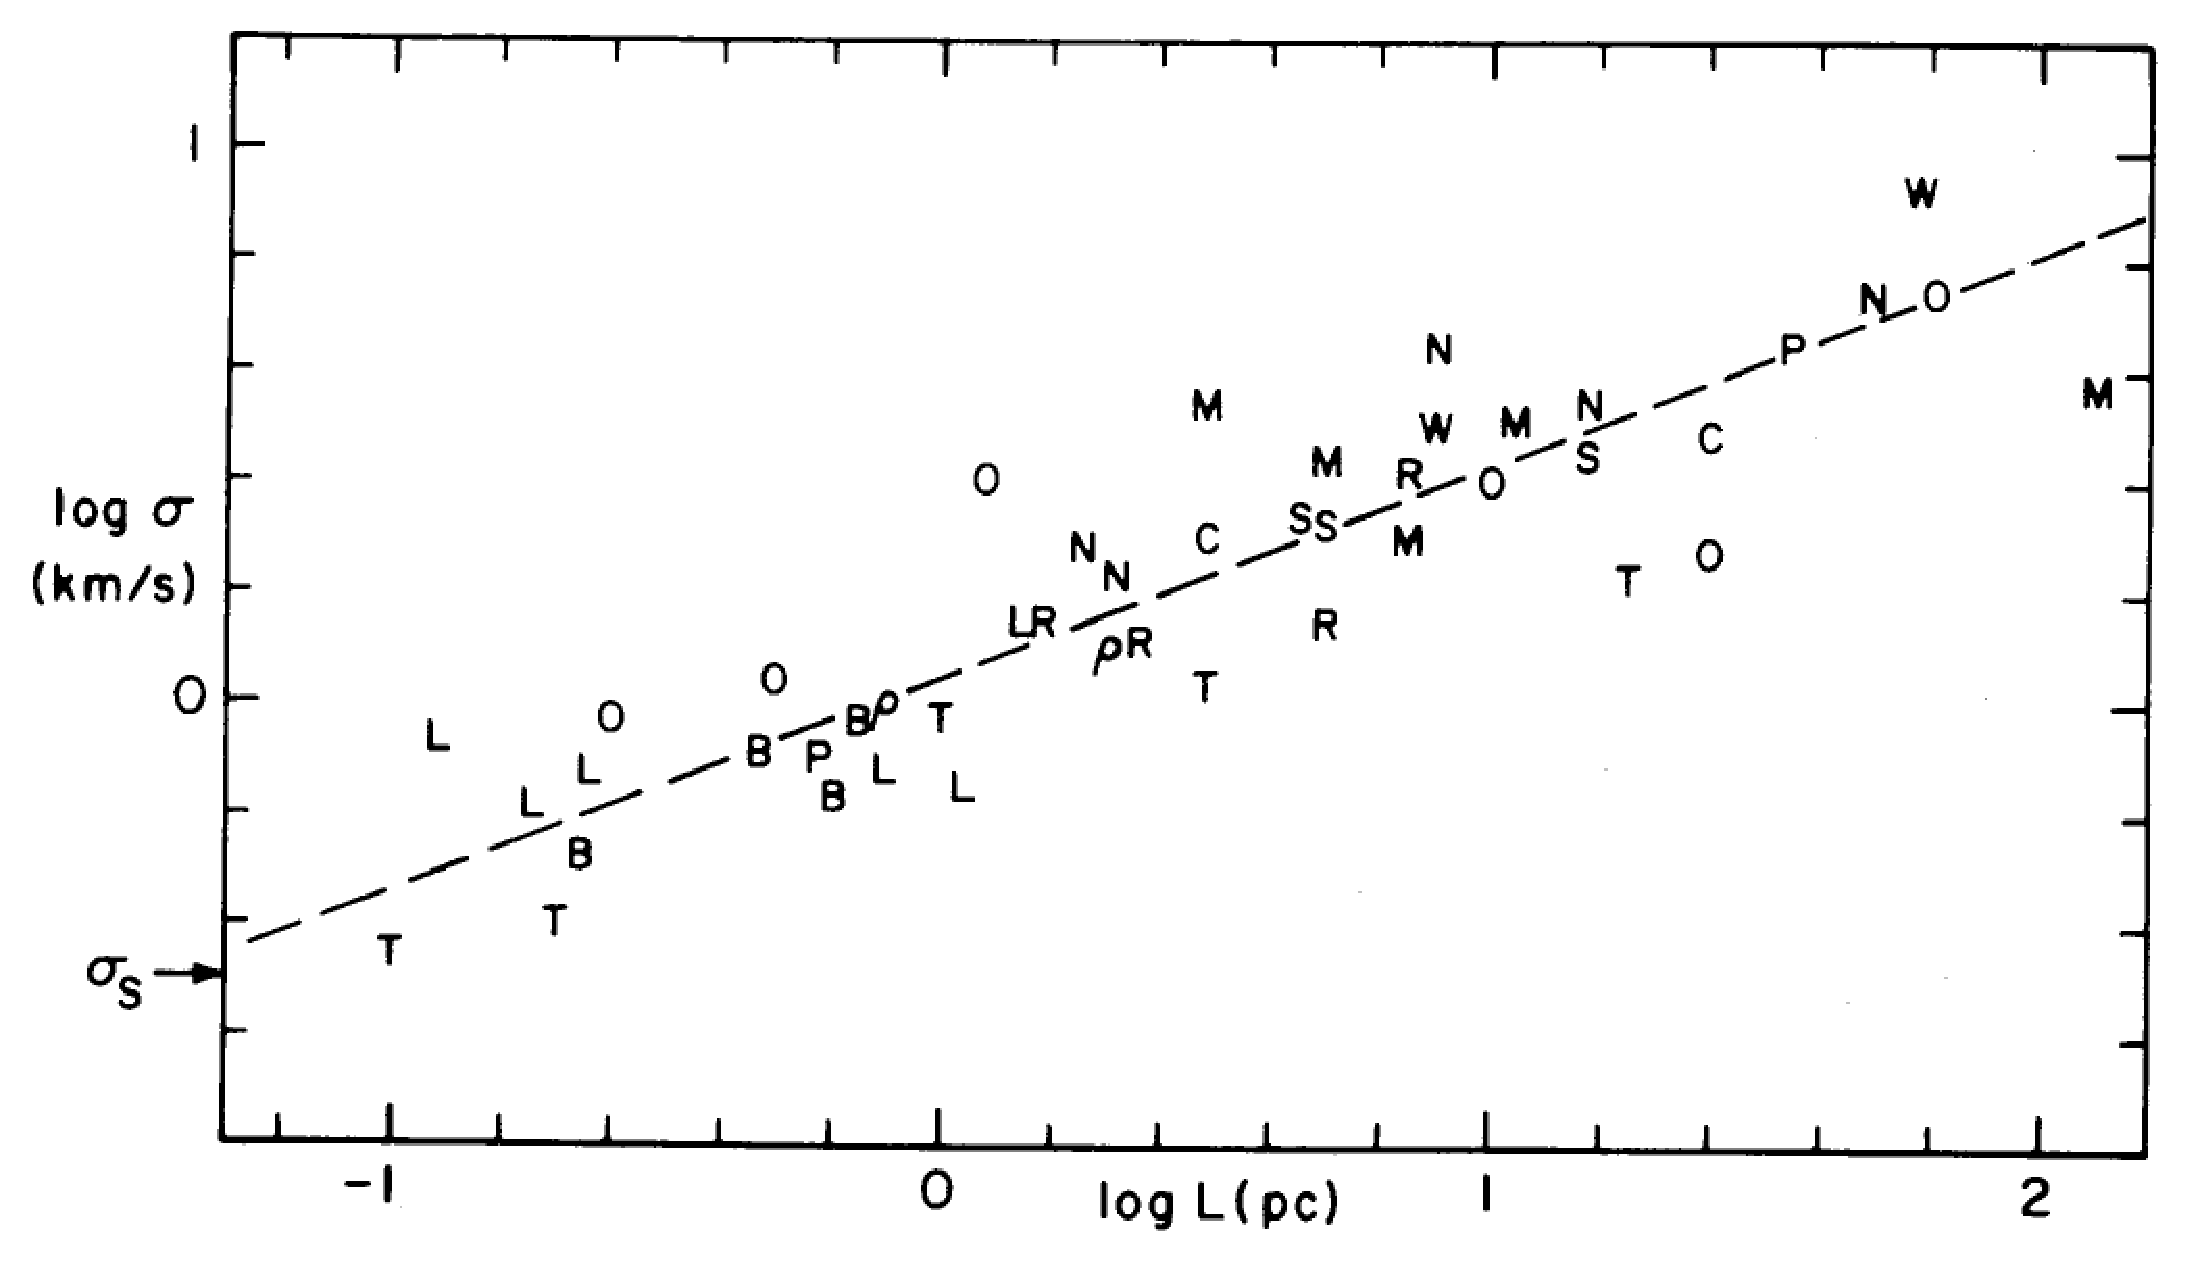
\includegraphics[width=8cm]{figures/larson}\\
	Slope of fit = 0.38
  \end{figure}
\end{frame}

\begin{frame}
	\frametitle{The Origins of Turbulence}
  \begin{itemize}
	  \item Turbulence decays in a few free-fall times
	  \item What keeps it going?
  \end{itemize}
\end{frame}

\begin{frame}
	\frametitle{Feedback from Massive Stars}
  \begin{figure}[t]
	\centering
	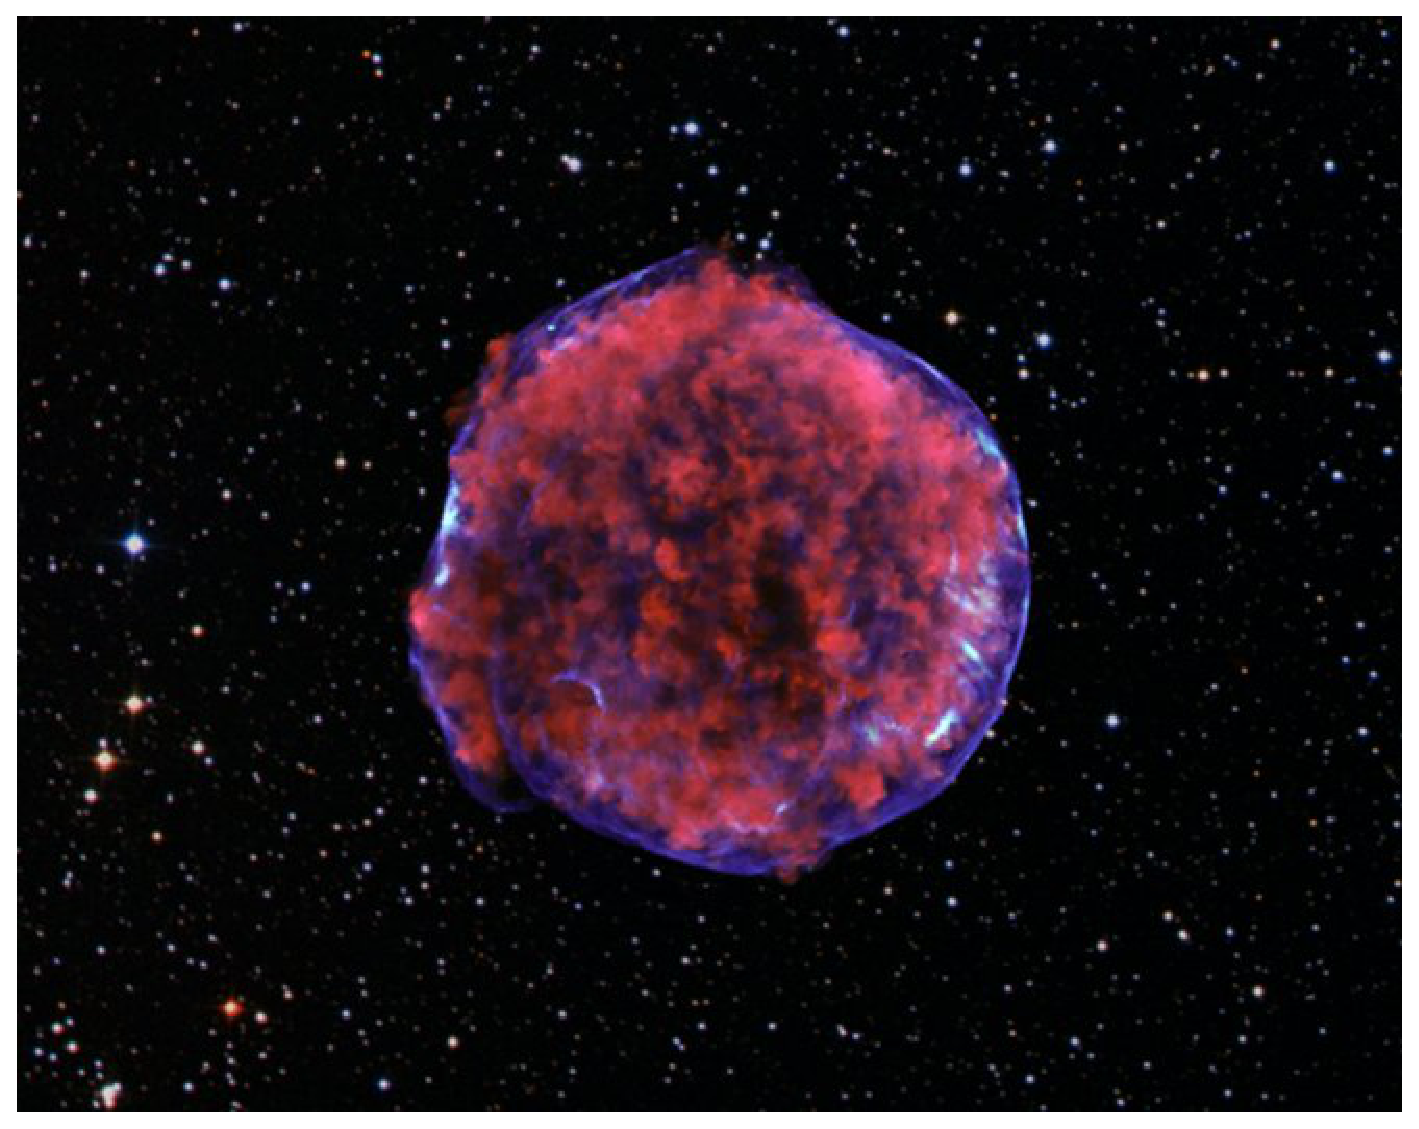
\includegraphics[width=8cm]{figures/tycho}\\
	A typical supernova injects $\approx 10^{51} erg$ on a scale of $\approx 50
	pc$
  \end{figure}
\end{frame}


\begin{frame}
	\frametitle{The Effects on Clouds}
  \begin{itemize}
	  \item Cloud Formation
	  \item Turbulent Support
	  \item Chemistry
	  \item Star formation \& Cloud fragmentation
  \end{itemize}
\end{frame}

\begin{frame}
	\frametitle{Cloud Formation}
  \begin{figure}[t]
	\centering
	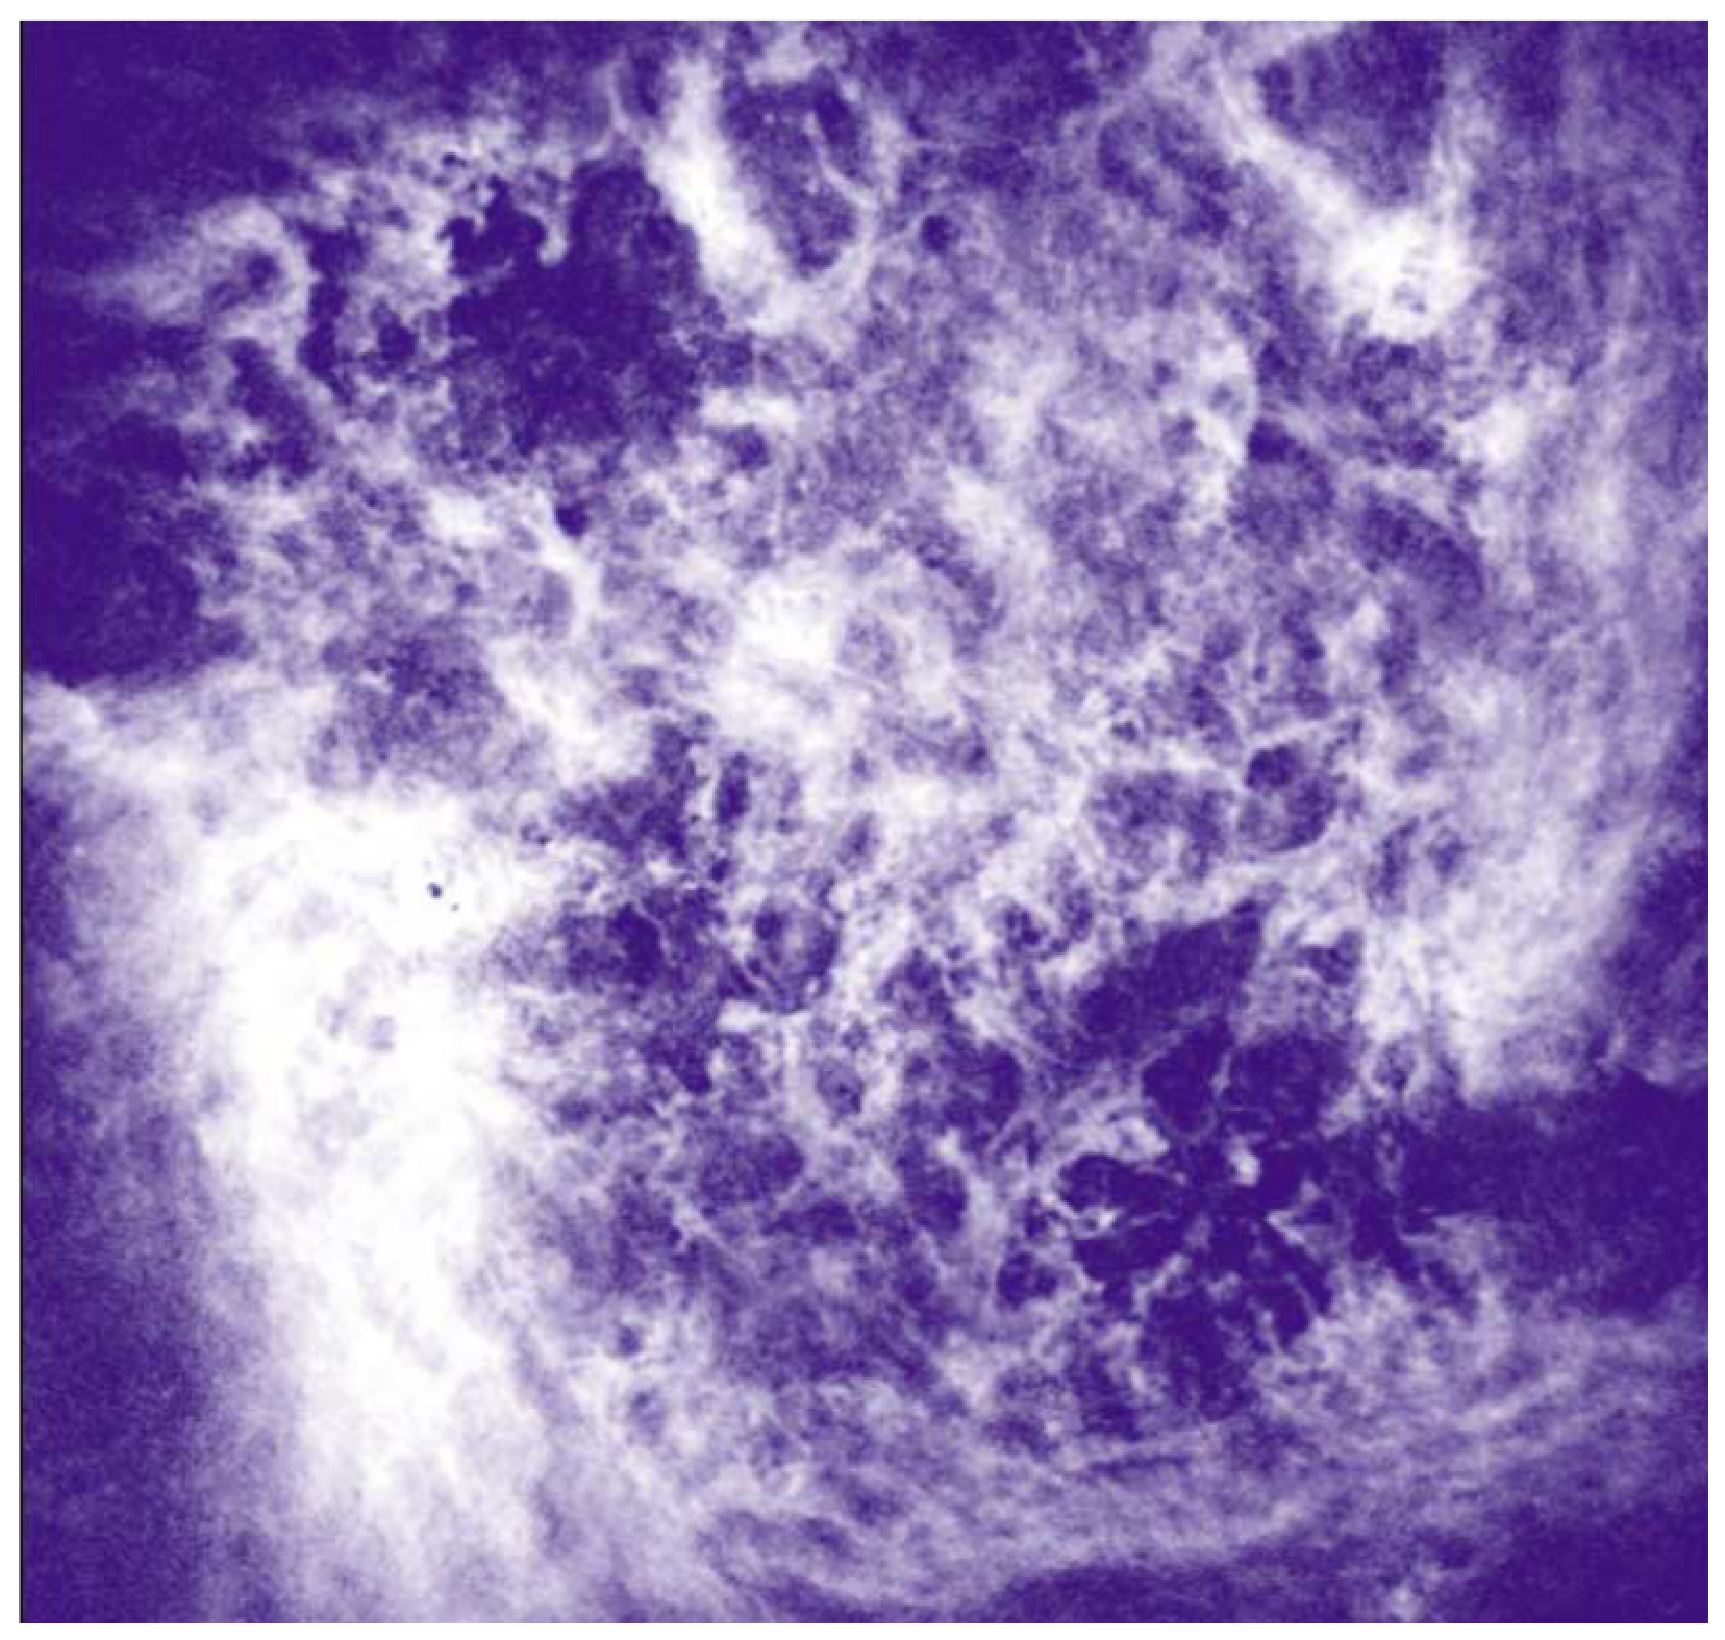
\includegraphics[width=7cm]{figures/LMC.eps}\\
	Molecular clouds can form rapidly from density perturbations in galactic-scale
	turbulence
  \end{figure}
\end{frame}

\begin{frame}
	\frametitle{Turbulent Support}
  \begin{itemize}
	  \item Why don't clouds just collapse?
	  \item Chandrasekhar 1951 proposed turbulent support:
    \begin{equation*}
		\lambda_J = 2\pi \sqrt{\frac{c_s^2}{4\pi G\rho}}
    \end{equation*}
    \begin{equation*}
		\lambda_{J-turbulent} = 2\pi \sqrt{\frac{c_s^2+u^2/3}{4\pi G\rho}}
    \end{equation*}
  \end{itemize}
\end{frame}

\begin{frame}
	\frametitle{Cloud Chemistry}
  \begin{itemize}
	  \item Turbulence generates density, temperature anisotropies
	  \item Turbulence can transport reactants and products between regions with
		  different physical conditions
  \begin{figure}[t]
	\centering
	\includegraphics[width=6cm]{figures/mixing}
  \end{figure}
  \end{itemize}
\end{frame}

\begin{frame}
	\frametitle{Chemical Transport}
  \begin{figure}[t]
	\centering
	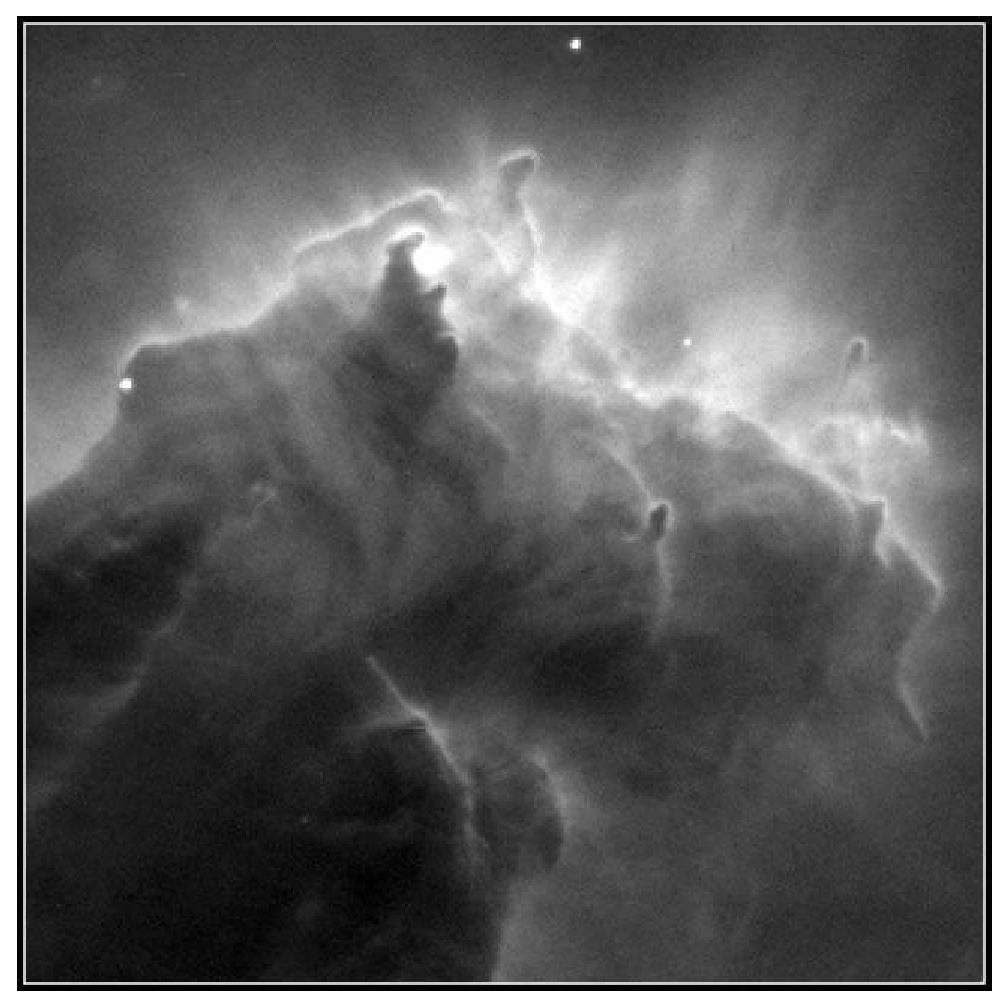
\includegraphics[width=7cm]{figures/evaporation}
  \end{figure}
\end{frame}

\begin{frame}
	\frametitle{Star Formation within Clouds}
  \begin{itemize}
	  \item Turbulence can make sub-cloud structures just as easily as it can
		  make clouds
	  \item These clumps have a characteristic mass function that should be
		  ``set" by turbulence
	  \item Hopkins 2013 has an analytic framework for generating mass functions
		  from turbulence.
  \end{itemize}
\end{frame}

\begin{frame}
	\frametitle{Turbulent Fragmentation}
  \begin{figure}[t]
	\centering
	\includegraphics[width=11cm]{figures/structure}
  \end{figure}
\end{frame}

\begin{frame}
	\frametitle{Turbulent Fragmentation}
  \begin{figure}[t]
	\centering
	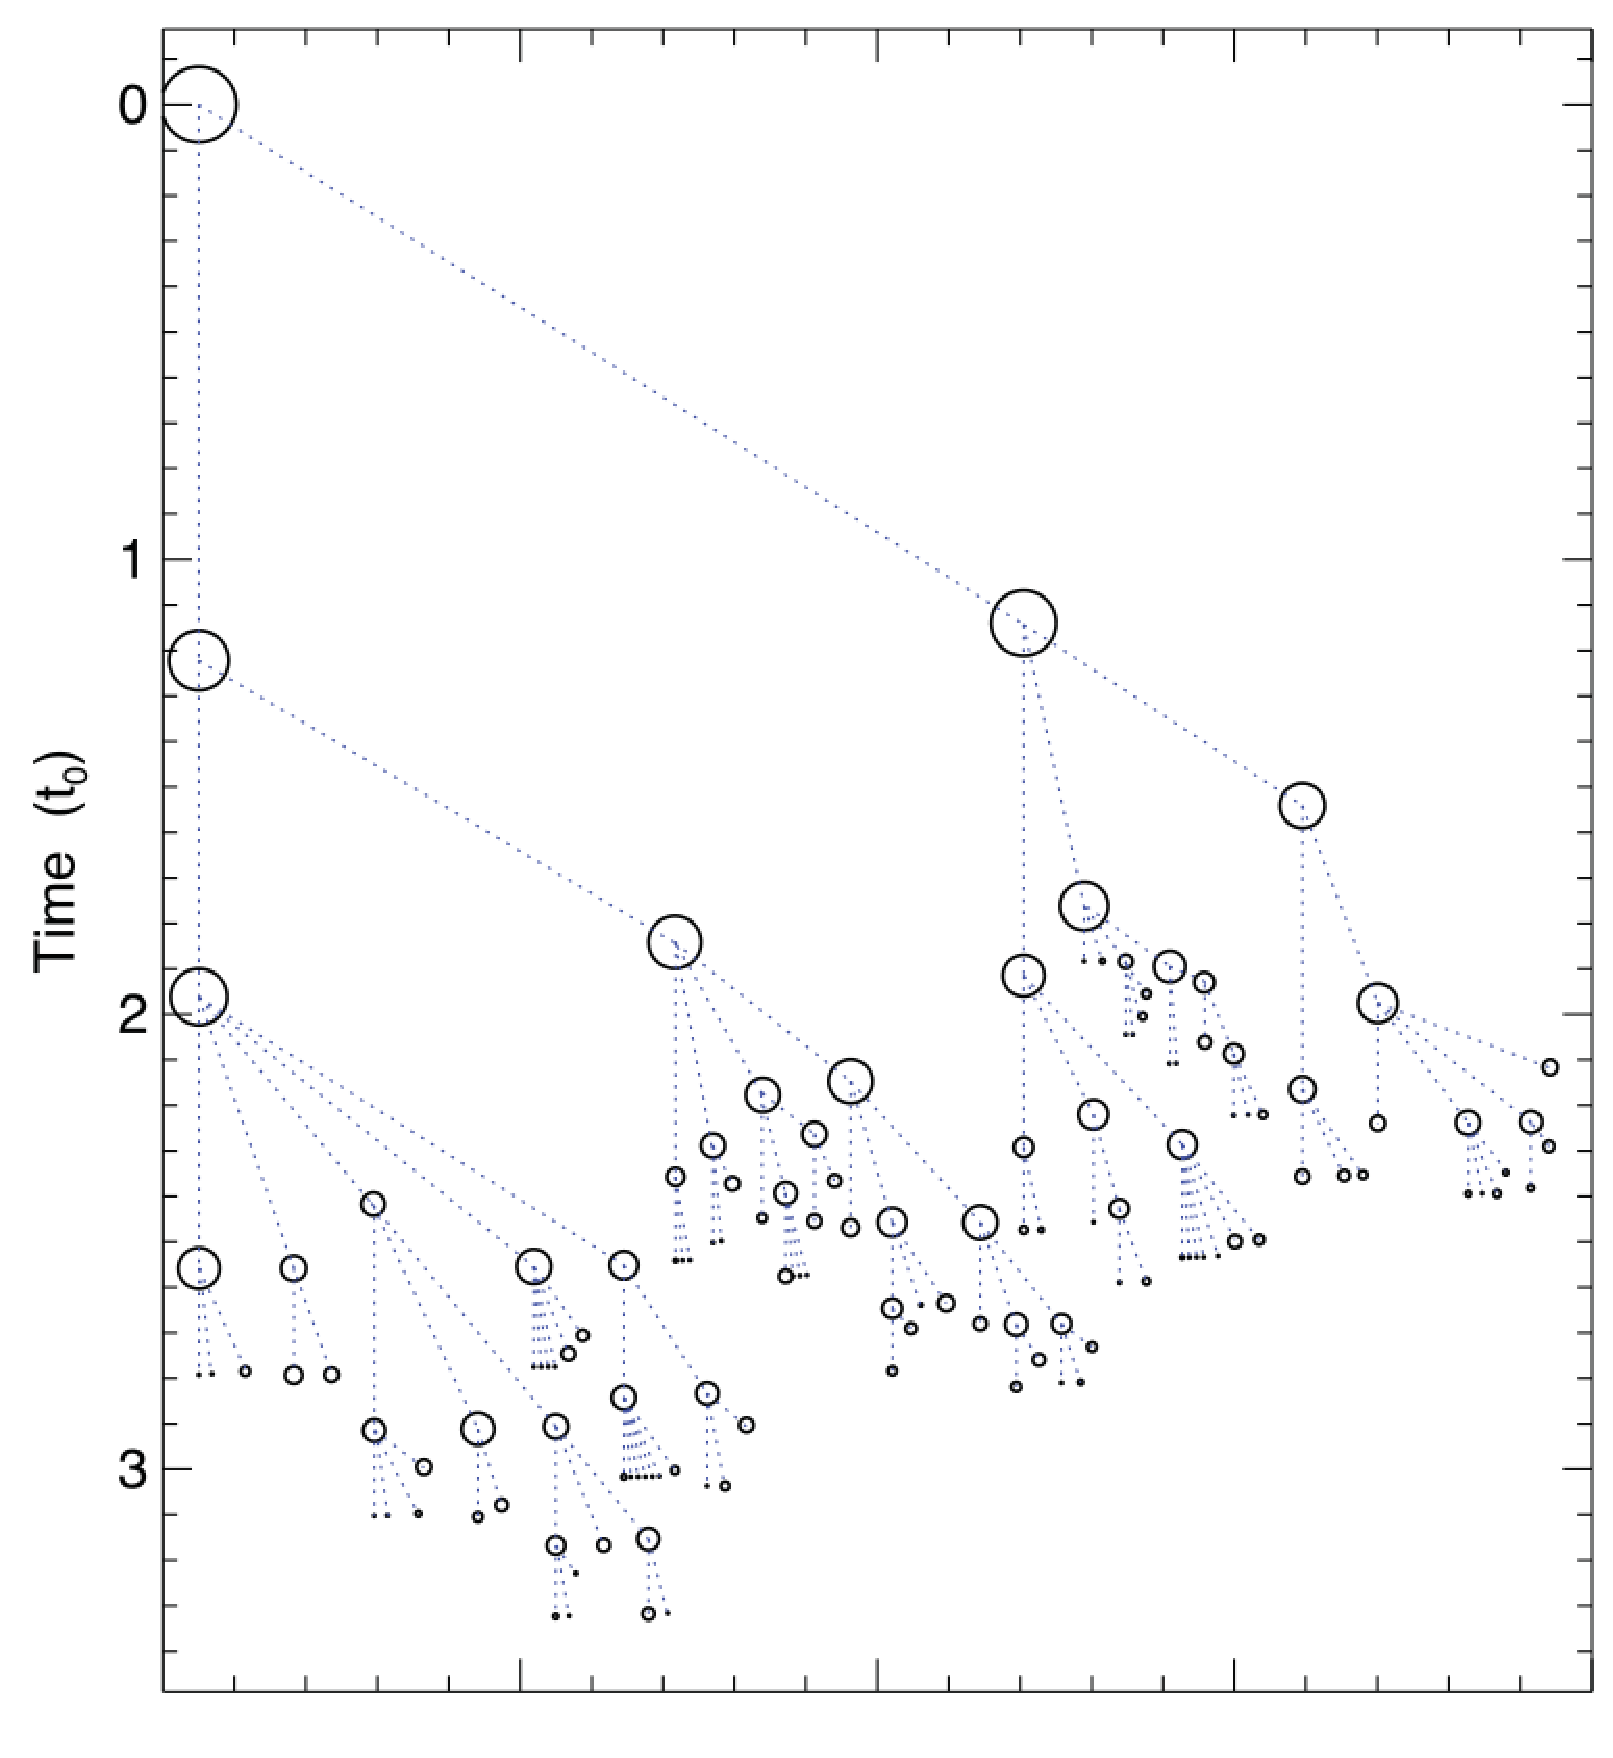
\includegraphics[width=7cm]{figures/fragtree}
  \end{figure}
\end{frame}

\begin{frame}
  \frametitle{Conclusions}
  \begin{itemize}
	  \item Turbulence can build and destroy molecular clouds
	  \item Turbulent pressure keeps clouds from rapidly collapsing to stars
	  \item Turbulence promotes chemical reactions within clouds
	  \item Turbulence may ultimately determine the mass functions for molecular
		  clouds and the structures within them (cores and stars)
  \end{itemize}
\end{frame}

\begin{frame}
  \frametitle{Questions?}
  \begin{figure}[t]
	\centering
	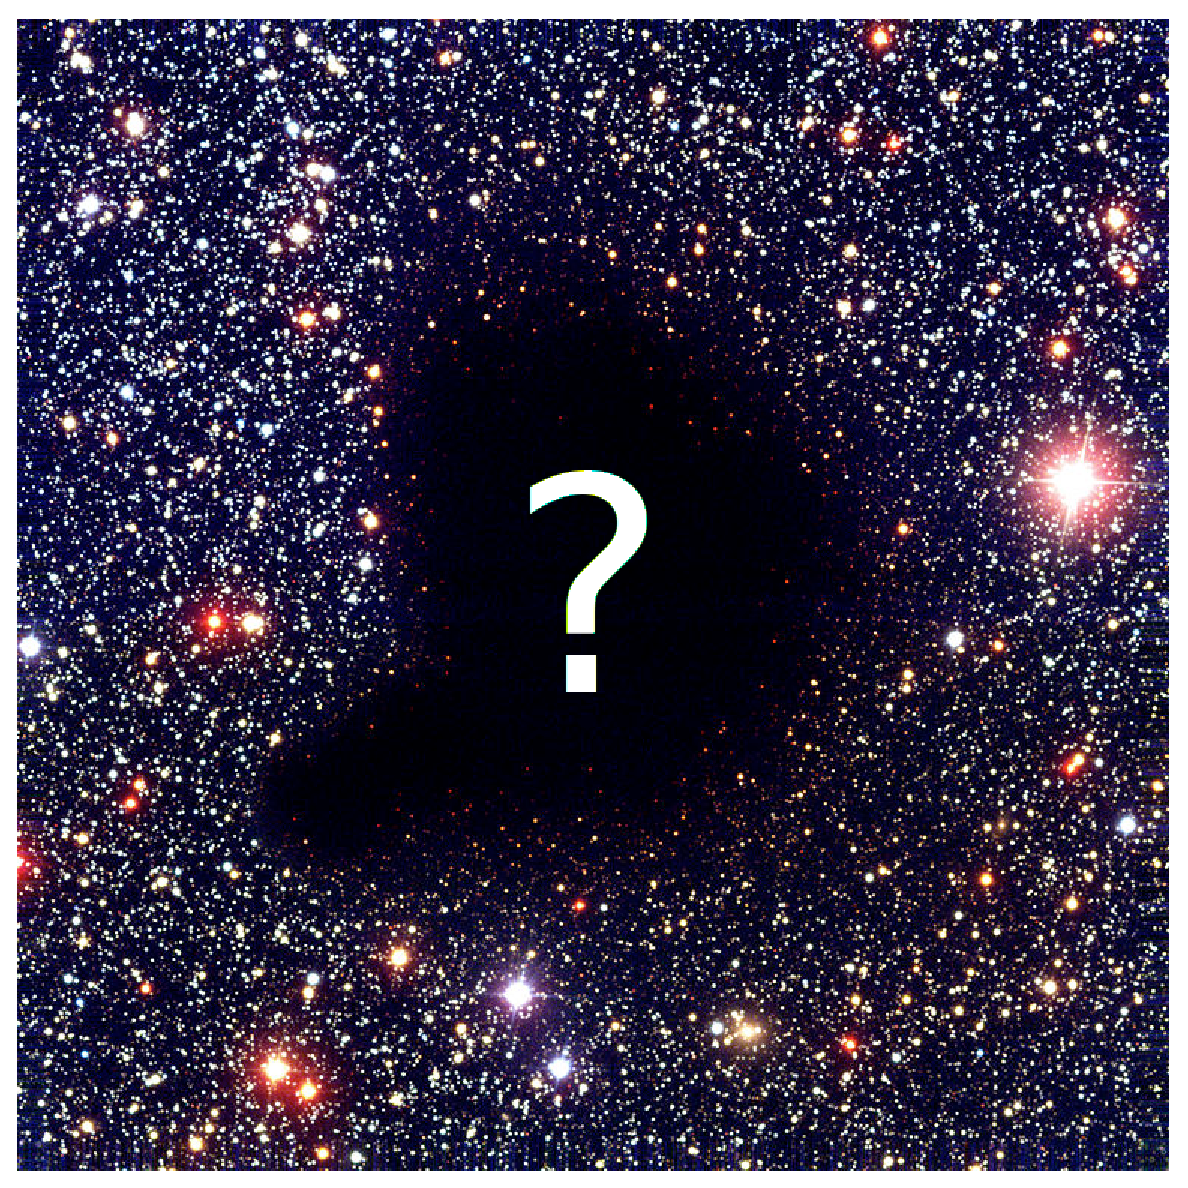
\includegraphics[width=6cm]{figures/bok}
  \end{figure}
\end{frame}
\end{document}
